\begin{pastexam}[label={px:gw3-113-ds-01}]{關務三等資訊處理 113 年 第一題}
（申論；20 分）

資料結構中的二元樹（binary tree）依其走訪節點的順序可以得出不同的運算表示式。給予一中序（inorder）表示式 FBACEIGJH
和後序（postorder）表示式 BCAFIHJGE，請說明並畫出其對應的二元樹。有一後序表示式 \texttt{36 12 / 10 23 - * 50 40 - +}
（此運算式中的數值均為二位數），利用堆疊運算其結果為何？（請勿只寫出最後結果，需詳細寫出堆疊內每一步的變化並說明）。
（20 分）
\end{pastexam}

\begin{pastsoln}
答案：二元樹畫在下面（根 E）；後序運算式的值是 $-29$。

（前半屬資結書第~7~章，後半的堆疊計算屬第~6~章。）

\textbf{重建二元樹}（資結書第~7.4~節、定理~7.4）：後序的最後一個是根；在中序裡找到根，左邊是左子樹、右邊是右子樹；後序
前面同樣個數的是左子樹，接著是右子樹。
\begin{itemize}
\item 根 $E$。 中序 F B A C $\mid$ E $\mid$ I G J H。 後序前 $4$ 個 B C A F 是左子樹，I H J G 是右子樹。
\item 左子樹：後序最後是 $F$，根 $F$。 中序 $F$ 在最前面，沒有左子樹；右子樹中序 B A C、後序 B C A，根 $A$，左子 $B$、
右子 $C$。
\item 右子樹：後序最後是 $G$，根 $G$。 中序 I $\mid$ G $\mid$ J H：左子 $I$；右子樹中序 J H、後序 H J，根 $J$，中序 $J$
在前，所以 $H$ 是 $J$ 的右子節點。
\end{itemize}
\begin{center}
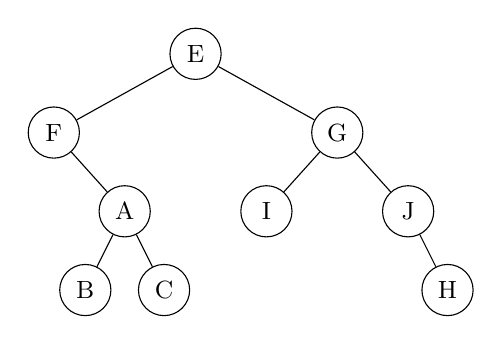
\begin{tikzpicture}[every node/.style={circle,draw,minimum size=6.5mm,inner sep=0pt,font=\small},
  level distance=10mm, level 1/.style={sibling distance=36mm}, level 2/.style={sibling distance=18mm},
  level 3/.style={sibling distance=10mm}]
\node {E}
  child {node {F} child[missing] child {node {A} child {node {B}} child {node {C}}}}
  child {node {G} child {node {I}} child {node {J} child[missing] child {node {H}}}};
\end{tikzpicture}
\end{center}
中序加後序可以唯一決定二元樹，所以這棵樹唯一。 檢查：中序 F B A C E I G J H、後序 B C A F I H J G E，和題目相同。

\textbf{後序運算式求值}（資結書第~6.3~節、虛擬碼~6.7）：由左到右讀，讀到數字就推入堆疊；讀到運算子就彈出兩個數，
先彈出的是\textbf{右}運算元 $b$、後彈出的是左運算元 $a$，算 $a \mathbin{\mathit{op}} b$ 後把結果推回。 讀完時堆疊裡剩下的
唯一一個數就是答案。
\begin{center}
\begin{tabular}{clll}
\toprule
步 & 讀入 & 動作 & 堆疊（左邊是底） \\
\midrule
1 & 36 & 推入 & 36 \\
2 & 12 & 推入 & 36, 12 \\
3 & / & 彈出 12、36，算 $36 / 12 = 3$，推入 & 3 \\
4 & 10 & 推入 & 3, 10 \\
5 & 23 & 推入 & 3, 10, 23 \\
6 & $-$ & 彈出 23、10，算 $10 - 23 = -13$，推入 & 3, $-13$ \\
7 & * & 彈出 $-13$、3，算 $3 \times (-13) = -39$，推入 & $-39$ \\
8 & 50 & 推入 & $-39$, 50 \\
9 & 40 & 推入 & $-39$, 50, 40 \\
10 & $-$ & 彈出 40、50，算 $50 - 40 = 10$，推入 & $-39$, 10 \\
11 & + & 彈出 10、$-39$，算 $-39 + 10 = -29$，推入 & $-29$ \\
\bottomrule
\end{tabular}
\end{center}
結果是 $-29$。 對應的中序運算式是 $(36 / 12) \times (10 - 23) + (50 - 40) = 3 \times (-13) + 10 = -29$。 注意減法和除法
不可交換，彈出的順序不能弄反：第 6 步是 $10 - 23$，不是 $23 - 10$。
\end{pastsoln}
